\wip
\section{Power over Ethernet}
\section{Spannungsregler}
\section{SMT}
Bei der klassischen THT-Technologie werden die Bauteilanschlüsse durch Löcher in der Platine gesteckt und mit kreisförmigen Lötpads auf der gegenüberliegenden Seite verlötet.
Im Gegensatz dazu sind bei SMD-Platinen Bauteile und Lötpads auf derselben Platinenseite, weshalb keine Bohrungen mehr erforderlich sind.
Die Bauteilanschlüsse werden flach mit dem rechteckigen Lötpad verbunden.
Die Verlötung findet mithilfe von Heißluft statt.
Die fertig bestückten Platinen werden in einen Reflow-Ofen gelegt und auf die Schmelztemperatur der Lötpaste erhitzt.

\subsection{Entwicklung}
In den 1960ern wurde die Oberflächenmontagetechnik (SMT) von IBM entwickelt und fand ihre ersten Anwendungen in den Saturn- und Apollo-Missionen.
In den 1970ern wurde die SMT erstmals genormt, wodurch sich die Technologie im kommerziellen Sektor verbreiten konnte.
Die SMT bietet gegenüber der herkömmlichen THT einige Vorteile:
\paragraph{Vorteile:}
\begin{itemize}
	\item Miniaturisierung, aufgrund der geringeren Größe der Bauteile können Platinen und somit auch Endgeräte kleiner und kompakter gebaut werden.
	\item Auch das Gewicht wird durch die Verkleinerung der Bauelemente stark reduziert.
	\item Der Bauteilabstand kann verkleinert werden, dadurch verbessert sich der Platzverbrauch weiter.
	\item Die Hochfrequenzeigenschaft wird durch die kürzeren Übertragungswege zwischen den Bauteilen verbessert.
	\item Die Fertigung der Platinen kann mit SMD besser automatisiert werden, da die Positionierung der Bauelement nicht so genau sein muss, wie bei THT.
	Die Bauteile werden beim Verlöten durch die Oberflächenspannung des Lötzinns in die korrekte Position gezogen.
	\item Einfache doppelseitige Bestückung von Platinen, da kein Platz von Anschlüssen von Bauteilen auf der anderen Platinenseite verbraucht wird.
\end{itemize}

\paragraph{Nachteile:}
\begin{itemize}
	\item Anschlüsse an der Unterseite von Bauteilen können nur durch Röntgen überprüft werden.
	\item Das Heißluftlötverfahren erhitzt nicht nur die Lötstelle, sondern das gesamte Bauteil.
 	Dadurch besteht ein höheres Risiko, dass dieses beim Anlöten zerstört wird.
 	\item Große Bauelemente benötigen zusätzliche Fixierung, da die Lötstelle der mechanischen Belastung nicht standhält.
	Aufgrund der vielen Vorteile gegenüber THT fand die SMT in der Digital- und Computertechnik anfänglich häufige Anwendung.
	Anfang der 1980er begannen die ersten Unternehmen mit der automatischen Fertigung von SMD-Platinen, wodurch die Herstellungskosten weiter gesenkt wurden.	
\end{itemize}

\subsection{Bauteilcodes}
Grundsätzlich werden alle elektronischen Bauteile in die beiden Untergruppen aktive und passive Bauelemente unterteilt.
Aktive Bauelemente können Signale verstärken oder erzeugen. Die benötigte Energie kommt aus einer zusätzlichen Versorgung durch elektrischer oder einer anderen Energieform. Beispiele für aktive Bauteile sind Transistoren, ICs, Photovoltaikzellen, …
Passive Bauelemente können im Gegensatz zu aktiven Bauteilen selbst keine Signale erzeugen oder verstärken. Sie benötigen keine zusätzliche Energieversorgung, um zu funktionieren. Beispiele für diese Art sind Widerstände, Kondensatoren und Spulen.

\subsubsection{Passive Bauteile}
Für passive Bauelemente gibt es vier wichtige Bezeichnungen:
\paragraph{Chip:}
Dies ist die Standard Bauform für unter anderem Keramik- und Tantal-Konden\-satoren, Induktivitäten sowie nichtlineare und lineare Widerstände.
Ein Chip ist ein quaderförmiges Bauteil, das auf der Platine aufliegt. In die Bezeichnung fließt nur die bauliche Größe ein.
Die Größe wird mit einem metrischen Code angegeben, z.B. „0603“, die Ziffer „06“ steht für die Länge und „03“ für die Breite.
In diesem Beispiel bedeutet das, dass das Bauteil 0,6 mm lang und 0,3 mm breit ist.
\begin{figure}[H]
	\centering
	\includegraphics{images/technische_grundlagen/chip.png}
	\caption{Chip-Bauform \cite[vgl.][]{vishay-chip}}
\end{figure}

\paragraph{MELF (Metal Electrode Faces):}
Die MELF Bauform ist im Gegensatz zur Chip-Bauform zylinderförmig, liegt aber ebenfalls flach auf der Platine auf.
Diese Bauform ist deutlich größer als die Chip Variante, dafür bietet sie elektrische Vorteile.
Die MELF Bauteile haben eine bessere Spannungsfestigkeit, höhere Impulsstrombelastbarkeit und eine bessere Temperaturstabilität.
Im Fehlerfall sind in dieser Bauweise die Widerstände so ausgelegt, dass sie in jedem Fall hochohmig werden und dadurch Schäden an anderen Bauteilen verhindern können.
Beim Lötvorgang hingegen kann es bei MELF Bauteilen dazu kommen, dass sie wegrollen. Daher werden sie meist vor dem Lötvorgang festgeklebt.
\begin{figure}[H]
	\centering
	\includegraphics{images/technische_grundlagen/melf.png}
	\caption{MELF-Bauform \cite[vgl.][]{vishay-melf}}
\end{figure}

\paragraph{SOD (Small Outline Diode):}
Wie der Name schon sagt ist das eine Gehäuseform, welche ausschließlich für Dioden verwendet wird. Die Bauteile sind entweder wie bei MELF zylindrisch (z.B. SOD-80 oder MiniMELF) oder quaderförmig mit Anschlussfahnen (z.B. SOD-123) ausgeführt.
\begin{figure}[H]
	\centering
	\includegraphics{images/technische_grundlagen/sod-123.png}
	\caption{SOD-123-Bauform \cite[vgl.][]{vishay-sod-123}}
\end{figure}

\paragraph{V-Chip (Vertical Chip):}
Ein V-Chip ist ebenfalls zylindrisch, jedoch werden diese Bauteile stehend montiert.
Diese Bauform wird häufig bei Aluminium-Elektrolytkondensator\-en verwendet und können dabei große Abmessungen erreichen.
\begin{figure}[H]
	\centering
	\includegraphics{images/technische_grundlagen/vchip.png}
	\caption{V-Chip-Bauform \cite[vgl.][]{vishay-vchip}}
\end{figure}

\subsubsection{Aktive Bauteile}
Für aktive Bauelemente (ICs) gibt es wesentlich mehr Bauformen und Bezeichnungen. Daher werden hier nur einige wichtige aufgeführt.
\paragraph{SOT (Small Outline Transistor):}
Diese Bauform wird ausschließlich für Transistoren verwendet. Sie hat drei oder vier Anschlüsse, wobei der vierte nur zum Abführen entstandener Wärme dient. Das Bauteil ist in dieser Bauform in einem quaderförmigen Kunststoff-Gehäuse verschweißt.
\begin{figure}[H]
	\centering
	\includegraphics{images/technische_grundlagen/sot-23.png}
	\caption{SOT-23-Bauform \cite[vgl.][]{vishay-sot}}
\end{figure}

\paragraph{SOIC (Small Outline Integrated Circuit):}
Bauteile in dieser Ausführung ähneln einem herkömmlichen DIP-Gehäuse, da der Anschlussabstand bei beiden Formen gleich groß ist. Dieser Gehäusetyp wird vor allem für ICs verwendet.
\begin{figure}[H]
	\centering
	\includegraphics{images/technische_grundlagen/soic.png}
	\caption{SOIC-Bauform \cite[vgl.][]{vishay-soic}}
\end{figure}

\paragraph{SOP (Small Outline Package):}
Dies ist eine kleinere Form der SOIC-Bauform und wird ebenso hauptsächlich für ICs verwendet. Diese Ausführung bekommt je nach Baugröße einen oder mehrere zusätzliche Buchstaben vorangestellt.
\begin{figure}[H]
	\centering
	\includegraphics{images/technische_grundlagen/sop.png}
	\caption{SOP-Bauform \cite[vgl.][]{vishay-sop}}
\end{figure}

%Entwicklung (zuerst tht, 1960 abgelöst durch smd, erfinder->IBM, Saturn- u. Apollo-Mission)
%Verwendung in Bereich Digitaltechnik, Raumfahrt; Bereiche für tht?
\subsection{Fehler}
\paragraph{Grabstein-Effekt:} %Bauteil hebt sich beim anlöten von der Platine
\begin{figure}[H]
	\centering
	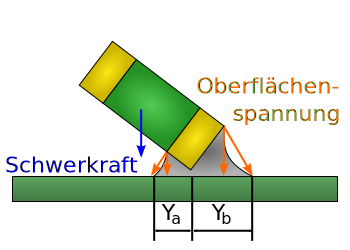
\includegraphics[width=.5\linewidth]{images/technische_grundlagen/grabsteinEffekt.png}%https://upload.wikimedia.org/wikipedia/commons/9/97/Tombstone_Effect_DE.svg
	\caption{Grabstein-Effekt}
\end{figure}

\paragraph{Popcorn-Effekt:} %aufgenommene Luftfeuchtigkeit expandiert beim Heißluftlöten und zerstört das bauteil
\begin{figure}[H]
	\centering
	\includegraphics[width=.5\linewidth]{images/technische_grundlagen/popcornEffekt.jpg}%https://upload.wikimedia.org/wikipedia/commons/9/97/PopcornBGA.jpg
	\caption{Popcorn-Effekt}
\end{figure}

\section{Serielle Schnittstellen}
\subsection{UART}
Universal Asynchronous Receiver/ Transmitter (UART) ist ein universell einsetzbarer elektronischer Baustein, der Systemeinheiten mit parallelem Übertragungsmodus an serielle Übertragungswege anpasst. 
Mit dem UART werden in Personal Computern (PC) die parallel anfallenden Daten in serielle Datenströme umgewandelt, die dann an den seriellen Schnittstellen (COM, LPT, IDE, usw.) für die angeschlossenen Peripheriegeräte und für die Datenübertragung über Modems zur Verfügung stehen. \cite{itwissen-uart}\par

Der UART-Datensatz besteht aus 11 Bit, einem Startbit, acht Datenbits, einem Paritätsbit und einem Stoppbit.
Der UART selbst besteht aus zwei FIFO-Puffern, die sende- und empfangsseitig die ein- und ausgehenden Datensignale zwischenspeichern.
Je nach Breite des Datenbusses gibt es Wandler für 8-Bit und 16-Bit mit Übertragungsraten von 19,2 kbit/s, 56 kbit/s (UART16450) und 128 kbit/s (UART16650D). \cite{itwissen-uart}\par
\begin{figure}[H]
	\centering
	\includegraphics[width=.9\linewidth]{images/technische_grundlagen/tide_uart_data.png}
	\caption{Aufbau eines UART-Frames \cite{tibbo-uart}}
\end{figure}

UART wurde für diese Anwendung ausgewählt, wegen der Einfachheit der Verdrahtung.
Die Kommunikation der Geräte findet über nur zwei Datenleitungen statt, dadurch werden Verbindungen zwischen der Platine und dem RPi eingespart.
UART wird vom RPi und Mikrocontroller unterstützt.


\subsection{Serial Peripheral Interface}
Das Serial Peripheral Interface, kurz SPI oder auch Micro Wire genannt, ist ein Bussystem bestehend aus drei Leitungen für eine serielle synchrone Datenübertragung zwischen verschiedenen ICs. \cite{mikrocontroller-spi}\par

Der Bus besteht aus folgenden Leitungen
\begin{itemize}
	\item MOSI (Master Out -> Slave In) auch SDO (Serial Data Out) oder DO
	\item MISO (Master In <- Slave Out) auch SDI (Serial Data In) oder DI
	\item SCK (Serial Clock) - Schiebetakt	
\end{itemize}
\cite{mikrocontroller-spi}

Zusätzlich zu diesen drei Leitungen wird für jeden Slave eine Slave Select (SS) oder auch Chip Select (CS) genannte Leitung benötigt, durch die der Master den Slave zur aktuellen Kommunikation selektiert. Dies geschieht dadurch, dass der Master die SS/CS-Leitung von High nach Low zieht. Oft ist mit dieser Aktivierung durch den Master auch eine Benachrichtigung für den Slave verbunden mit der ihm mitgeteilt wird, dass jetzt eine Nachricht beginnt, das nächste Byte also zum Beispiel als Kommando aufzufassen ist. \cite{mikrocontroller-spi}\par

Die Übertragung geschieht so, dass der Master seine Datenleitung (MOSI) auf den Pegel des nächsten Bits bringt und dann an der SCK Leitung einen Puls ausgibt. Gleichzeitig wird vom Master der Pegel an der Datenleitung vom Slave zum Master überwacht und ihr Zustand als nächstes einzulesendes Bit aufgefasst. Üblicherweise gibt es zumindest beim Master mehrere Einstellungen, die festlegen, welches der Grundzustand dieser SCK Leitung sein soll und welche Flanke des Taktes zur Datenübernahme herzunehmen ist (die steigende oder die fallende). Bei einigen Slaves ist diese Einstellung ebenfalls möglich, oft ist es aber so, dass per SPI anzusprechende IC eine feste Einstellung benutzen, an die sich der Master anpassen muss. \cite{mikrocontroller-spi}\par

Für den SPI-Bus gibt es kein festgelegtes Protokoll. Die Taktpolarität (CPOL) und Phase (CPHA) können ebenfalls von Slave zu Slave unterschiedlich sein. Der SPI-Bus kann mit einer Taktfrequenz von vielen Megahertz betrieben werden. Es gibt viele verschiedene ICs die als Slave an dem SPI-Bus betrieben werden können, diese gehen von einfachen Schieberegistern bis hin zu RTCs oder Displaytreibern mit vorgegebenem Protokoll. Unter anderem werden die meisten AVR-Microcontroller von Atmel über SPI programmiert. \cite{mikrocontroller-spi}\par

\section{Audio-Verstärker Class D}
Mit Class-D wird ein bestimmtes Schaltungsdesign von Audio-Verstärkern bezeichnet, die ein PWM-Signal (englisch PWM = Pulse Width Modulation, Pulsbreitenmodulation) erzeugen und daher auch als PWM-Verstärker bekannt sind. \cite{fairaudio-classd}\par

Es hat sich vielerorts heute eingebürgert, „Class-D“ mit „digital“ zu übersetzen. Historisch war „D“ jedoch als Kategorie an der Reihe, nachdem die Buchstaben „A“, „B“ und „C“ bereits für andere Verstärkerklassen vergeben waren, die früher aufkamen. Heute nutzen einige Class-D-Designs intern auch Digitaltechnik. Dies kann durch die Zusatzeigenschaft „digitally controlled“ (digital kontrolliert) ausgedrückt werden. Das PWM-Signal am Verstärkerausgang ist dabei in jedem Fall als ein Analogsignal zu sehen, welches nach Tiefpassfilterung direkt zur Ansteuerung eines Lautsprechers verwendet werden kann. \cite{fairaudio-classd}\par

Da auch von Schaltverstärkern gesprochen wird und tatsächlich die Ausgangsstufe entweder „An“ oder „Aus“ ist, liegt die vereinfachende Analogie zur Digitaltechnik aber nahe: Bei dieser wird ebenfalls mit binären Werten (0/1 – Aus/An) gearbeitet (dazu weiter unten mehr). Ein wesentliches Merkmal der Digitaltechnik – die festgelegte Anzahl von Stufen bei Fehlen von Zwischenwerten (die Wortbreite, z. B. 16 Bit) – gibt es bei Class-D-Schaltungen aber nicht. Bei ihr sind (zumindest theoretisch) unendlich viele Zwischenstufen möglich, auch wenn in der Praxis sicherlich Restriktionen auftreten. \cite{fairaudio-classd}\par

Eine Class-D Schaltung lässt sich schematisch in drei Bereiche unterteilen:
\begin{enumerate}
	\item Der erste Bereich besteht aus dem Eingang für das Audiosignal, einem Signal-Generator (Dreieck) und einem sogenannten Komparator (Comp).
	\item Die eigentliche Schalt-Verstärkungsstufe enthält einen Controller und die Transistoren (in der Regel MOSFETs), die das vom Komparator kommende PWM-Signal verstärken.
	\item Das Tiefpass-Filter (hohe Frequenzen werden herausgefiltert), welches das am Eingang generierte Signal (die Trägerfrequenz) wieder herausfiltert.	
\end{enumerate}
\cite{fairaudio-classd}
\begin{figure}[H]
	\centering
	\includegraphics[width=.9\linewidth]{images/technische_grundlagen/class-d-schematisch.png}
	\caption{Schematische Darstellung Class-D \cite{fairaudio-classd}}
\end{figure}
%falls noch mehr text benötigt wird: erklärungen auf website